%----------------------------------------------------------------------------
\chapter{A lekérdező program}\label{sect:Ellaboration}
%----------------------------------------------------------------------------
\section{Fejlesztés menetének áttekintése}
Első lépésként tehát a bevezetőben megfogalmazott problémák megoldása érdekében,
készítettem egy saját magas szintű lekérdező nyelvet az Essbase-hez, mégpedig
úgy, hogy a riport valamint az mdx nyelv összetevői alapján megfogalmaztam
Xtextben egy metamodellt, amit már az Xtext ezután tud értelmezni, és egy
konkrét lekérdezés megírásánál tudja azt validálni.

Majd ezek után az általam újonnan létrehozott nyelvbe, létrehoztam saját
lekérdezést, amit amiben meg lehet nézni a havi kimutatást, költségeket.

Ezután készítettem egy szerkesztőt, amibe a fejlesztők tudnak dolgozni, ehhez
egy Eclipse pugint csináltam, beépítve az Xtext nyelvtan elemző programomat. 

A program indítás után áttranszformálja a megírt lekérdezést olyan forráskóddá
amit az Essbase értelmezni tud, majd hálózaton keresztül elkéri azt egy
objektumba, amivel utána lehet dolgozni. A visszakapott objektumot ezután, a
megfelelő parancsal, ezután meg lehet jeleníteni, riportolni, egy Latex pdf-be,
amit a program generál.

 \begin{figure}[!ht]
\centering
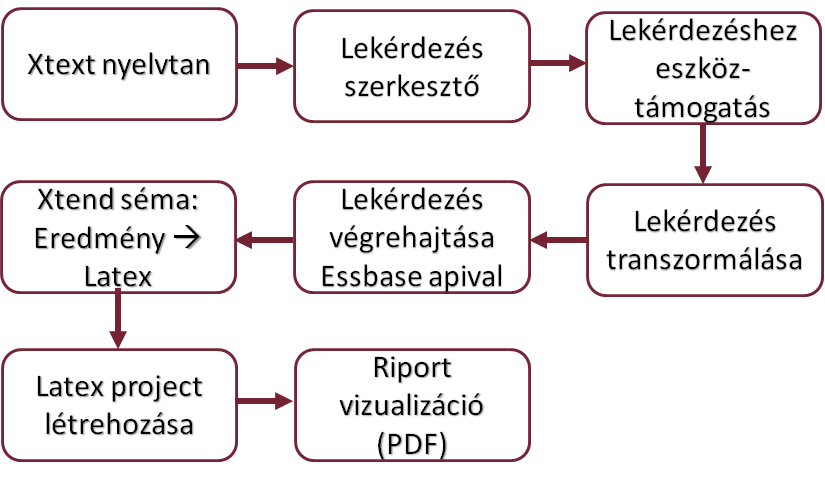
\includegraphics[width=120mm, keepaspectratio]{figures/overview.png}
\caption{A folyamat áttekintése} 
\label{fig:Overview}
\end{figure}

\section{A lekérdező nyelv bemutatása}

\begin{lstlisting}[language=java,morekeywords={dim,group,row,link,reportParameter,report,query},alsoletter={-},breaklines=true]
SajatQuery1=query {
	{SUPEMPTYROWS}
{DECIMAL 10}
{TABDELIMIT}
{ROWREPEAT}
{SUPBRACKETS}
{SUPCOMMAS}
{NOINDENTGEN}

dim ktg "Input_KN_Koltsegnem"
dim obj "Input_Objektum"
group objects "Input_Objektumok"
group ktgs "Input_KN_Koltsegnemek"

row {obj,ktg}
link {objects,obj}
link {ktgs,ktg}
reportParameter {"UGYF"}   }
report SajatQuery1
\end{lstlisting}

\section{Validációs módszerek}








